% Generated by src/eval/e9HandoverPoint.js -- do not edit by hand.
\begin{figure}[htbp]
    \centering
    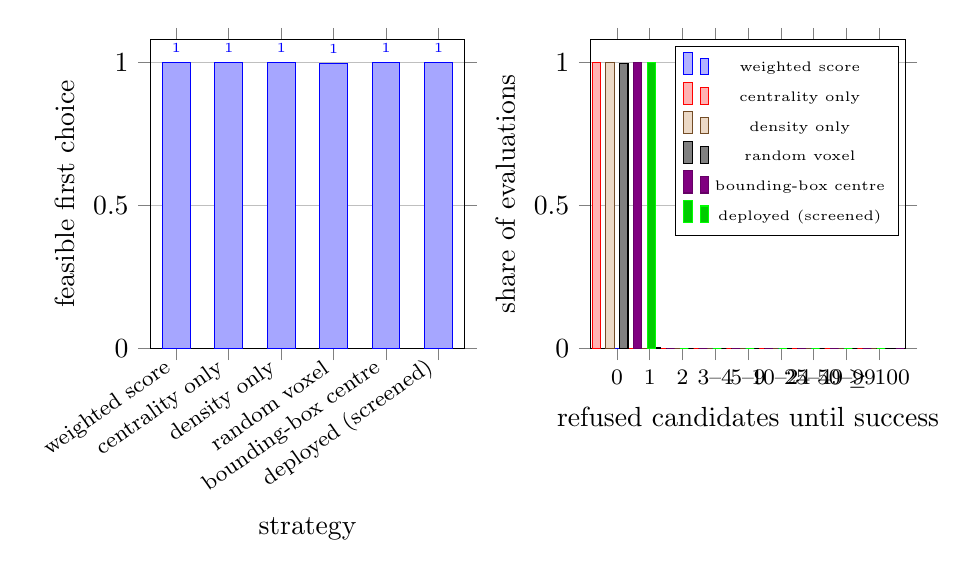
\begin{tikzpicture}
        \begin{axis}[
            name=feasibility, width=0.46\textwidth, height=5.5cm,
            ybar, bar width=10pt, ymin=0, ymax=1.08,
            ylabel={feasible first choice}, xlabel={strategy},
            symbolic x coords={s0, s1, s2, s3, s4, s5}, xtick=data,
            xticklabels={weighted score, centrality only, density only, random voxel, bounding-box centre, deployed (screened)},
            xticklabel style={rotate=35, anchor=east, font=\footnotesize},
            nodes near coords, every node near coord/.append style={font=\tiny},
            ymajorgrids, tick align=outside
        ]
            \addplot+[fill=blue!35] coordinates {(s0, 1.0000) (s1, 1.0000) (s2, 1.0000) (s3, 0.9970) (s4, 1.0000) (s5, 1.0000)};
        \end{axis}
        \begin{axis}[
            at={(feasibility.south east)}, xshift=1.6cm, anchor=south west,
            width=0.46\textwidth, height=5.5cm,
            ybar, bar width=3pt, ymin=0, ymax=1.08,
            ylabel={share of evaluations}, xlabel={refused candidates until success},
            symbolic x coords={b0, b1, b2, b3, b4, b5, b6, b7, b8}, xtick=data,
            xticklabels={0, 1, 2, 3--4, 5--9, 10--24, 25--49, 50--99, $\geq$ 100},
            xticklabel style={font=\footnotesize},
            legend style={font=\tiny, at={(0.98,0.98)}, anchor=north east},
            ymajorgrids, tick align=outside
        ]
            \addplot coordinates {(b0, 1.0000) (b1, 0.0000) (b2, 0.0000) (b3, 0.0000) (b4, 0.0000) (b5, 0.0000) (b6, 0.0000) (b7, 0.0000) (b8, 0.0000)};
            \addlegendentry{weighted score}
            \addplot coordinates {(b0, 1.0000) (b1, 0.0000) (b2, 0.0000) (b3, 0.0000) (b4, 0.0000) (b5, 0.0000) (b6, 0.0000) (b7, 0.0000) (b8, 0.0000)};
            \addlegendentry{centrality only}
            \addplot coordinates {(b0, 1.0000) (b1, 0.0000) (b2, 0.0000) (b3, 0.0000) (b4, 0.0000) (b5, 0.0000) (b6, 0.0000) (b7, 0.0000) (b8, 0.0000)};
            \addlegendentry{density only}
            \addplot coordinates {(b0, 0.9970) (b1, 0.0030) (b2, 0.0000) (b3, 0.0000) (b4, 0.0000) (b5, 0.0000) (b6, 0.0000) (b7, 0.0000) (b8, 0.0000)};
            \addlegendentry{random voxel}
            \addplot coordinates {(b0, 1.0000) (b1, 0.0000) (b2, 0.0000) (b3, 0.0000) (b4, 0.0000) (b5, 0.0000) (b6, 0.0000) (b7, 0.0000) (b8, 0.0000)};
            \addlegendentry{bounding-box centre}
            \addplot coordinates {(b0, 1.0000) (b1, 0.0000) (b2, 0.0000) (b3, 0.0000) (b4, 0.0000) (b5, 0.0000) (b6, 0.0000) (b7, 0.0000) (b8, 0.0000)};
            \addlegendentry{deployed (screened)}
        \end{axis}
    \end{tikzpicture}
    \caption{E9: left, the rate at which the first point a strategy proposes can be served by both arms; right, how many candidates the cell has to refuse before a feasible point stands. All strategies rank the unscreened height band; the deployed pipeline screens it first, so its feasibility is one by construction and its refusal count zero.}
    \label{fig:exp_e9}
\end{figure}
